

%% CAP High School Prize Examination
%%----------------------------------------


%% this section contains 40 problems


%% CAP Exam 2015
%%----------------------------------------
\element{cap}{ %% cap-A4
\begin{question}{CAP-A-2015-q16}
    A ball is placed on a massless spring that is held at an angle of $\theta$ with respect to the horizontal. 
    The spring is then compressed a distance of $x$ and released. 
    When the ball reaches the maximum height of its trajectory,
        it is traveling at a speed $v$.
    Then a different ball, weighing four times as much as the first,
        is placed on the spring which is still at an angle $\theta$. 
    The spring is again compressed a distance $x$ and released. 
    Compared to the first ball, the second ball reaches a maximum height that is:
    \begin{choices}
        \wrongchoice{$\sin^2\theta$ times as high.}
      \correctchoice{$\dfrac{1}{4}$ times as high.}
        \wrongchoice{$\dfrac{v^2 g}{x}$ times as high.}
        \wrongchoice{4 times higher.}
    \end{choices}
\end{question}
}


%% CAP Exam 2014
%%----------------------------------------
\element{cap}{ %% cap-A4
\begin{question}{CAP-A-2014-q04}
    The friction force acting on a bicycle is \SI{20}{\newton}. 
    What power does a cyclist need in order to travel at \SI{18}{\kilo\meter\per\hour}?
    \begin{multicols}{2}
    \begin{choices}
        \wrongchoice{\SI{50}{\watt}}
      \correctchoice{\SI{100}{\watt}}
        \wrongchoice{\SI{1800}{\watt}}
        \wrongchoice{\SI{3600}{\watt}}
    \end{choices}
    \end{multicols}
\end{question}
}

\element{cap}{ %% cap-A4
\begin{question}{CAP-A-2014-q14}
    To submerge a block of wood which is less dense than water,
        one needs to exert a force downward which does a positive amount of work on the block. 
    Which of the following is correct for this situation to occur?
    \begin{choices}
        \wrongchoice{The work done by the external force is stored as potential energy in the block.}
        \wrongchoice{The block is moving downward, therefore its potential energy is decreasing, thus the work done by the external force is all converted to heat, due to friction.}
        \wrongchoice{The work done by external force is all stored as kinetic energy in the block.}
      \correctchoice{The potential energy of the water is increased while the potential energy of the block is decreased.}
        \wrongchoice{The total energy of the block is conserved.}
        \wrongchoice{The total energy of the block and water is conserved.}
    \end{choices}
\end{question}
}

\element{cap}{ %% cap-A4
\begin{question}{CAP-A-2014-q21}
    A ball is dropped to the Earth from a height of \SI{2}{\meter}.
    Neglecting the air resistance,
        which one of the following graphs represents the kinetic energy of the ball vs. time?
    \begin{multicols}{2}
    \begin{choices}
        \AMCboxDimensions{down=-2.5em}
        \wrongchoice{
            \begin{tikzpicture}
                \begin{axis}[
                    axis y line=left, 
                    axis x line=bottom, 
                    axis line style={->},
                    xlabel={time},
                    xtick=\empty,
                    ylabel={kinetic energy},
                    ytick=\empty,
                    xmin=0,xmax=11,
                    ymin=0,ymax=11,
                    width=1.0\columnwidth,
                ]
                \addplot[line width=1pt] plot coordinates { (0,3) (10,3) };
                \end{axis}
            \end{tikzpicture}
        }
        \wrongchoice{
            \begin{tikzpicture}
                \begin{axis}[
                    axis y line=left, 
                    axis x line=bottom, 
                    axis line style={->},
                    xlabel={time},
                    xtick=\empty,
                    ylabel={kinetic energy},
                    ytick=\empty,
                    xmin=0,xmax=11,
                    ymin=0,ymax=11,
                    width=1.0\columnwidth,
                ]
                \addplot[line width=1pt] plot coordinates { (0,0) (10,10) };
                \end{axis}
            \end{tikzpicture}
        }
        %% ANS is C
        \correctchoice{
            \begin{tikzpicture}
                \begin{axis}[
                    axis y line=left, 
                    axis x line=bottom, 
                    axis line style={->},
                    xlabel={time},
                    xtick=\empty,
                    ylabel={kinetic energy},
                    ytick=\empty,
                    xmin=0,xmax=11,
                    ymin=0,ymax=11,
                    width=1.0\columnwidth,
                ]
                \addplot[line width=1pt,domain=0:10] { 0.1*x*x };
                \end{axis}
            \end{tikzpicture}
        }
        \wrongchoice{
            \begin{tikzpicture}
                \begin{axis}[
                    axis y line=left, 
                    axis x line=bottom, 
                    axis line style={->},
                    xlabel={time},
                    xtick=\empty,
                    ylabel={kinetic energy},
                    ytick=\empty,
                    xmin=0,xmax=11,
                    ymin=0,ymax=11,
                    width=1.0\columnwidth,
                ]
                \addplot[line width=1pt,domain=0:10] { sqrt(10) * sqrt(x) };
                \end{axis}
            \end{tikzpicture}
        }
    \end{choices}
    \end{multicols}
\end{question}
}


%% CAP Exam 2012
%%----------------------------------------
\element{cap}{ %% cap-A4
\begin{question}{CAP-A-2012-q08}
    A car starts to move at time $t=0$. 
    If the engine of the car is able to provide constant power,
        which of the following statements is correct about the speed of car at the beginning of the motion?
    \begin{choices}
        \wrongchoice{The speed is constant.}
        \wrongchoice{The speed increases proportionally to time passed ($v \propto t$).}
      \correctchoice{The speed increases as the square root of time ($v \propto \sqrt{t}$).}
        \wrongchoice{The speed increases as time squared ($v \propto t^2$).}
    \end{choices}
\end{question}
}


%% CAP Exam 2011
%%----------------------------------------
\element{cap}{ %% cap-A4
\begin{question}{CAP-A-2011-q22}
    Many cars are now equipped with anti-lock brakes (ABS),
        which prevents locking of the wheels during emergency braking. 
    What is the main advantage?
    \begin{choices}
        \wrongchoice{This saves the tires. Otherwise too much rubber is left on the road.}
        \wrongchoice{Provides more control over the car but stopping distance increases slightly.}
        \wrongchoice{This leads to a shorter stopping distance because tires exert rolling friction which is larger than kinetic friction.}
        \wrongchoice{This leads to a shorter stopping distance because tires exert rolling friction which is larger than static friction.}
      \correctchoice{This leads to a shorter stopping distance because tires exert static friction which is larger than kinetic friction.}
    \end{choices}
\end{question}
}


%% CAP Exam 2010
%%----------------------------------------
\element{cap}{ %% cap-A4
\begin{question}{CAP-A-2010-q18}
    A fish swimming in water with constant velocity $v_0$ experiences a viscous drag force that is proportional to the square of its velocity (\emph{i.e.} $F_{\text{drag}}\propto v^2$).
    If the fish doubles its velocity,
        then the thrust force $F$ that it must generate to maintain this new velocity is related to the fish's original thrust force $F_0$ via:
    \begin{multicols}{2}
    \begin{choices}
        \wrongchoice{$F = 2 F_0$}
        \wrongchoice{$F = \sqrt{2} F_0$}
      \correctchoice{$F = 4 F_0$}
        \wrongchoice{$F = F_0^2$}
        \wrongchoice{none of the provided}
    \end{choices}
    \end{multicols}
\end{question}
}


%% CAP Exam 2009
%%----------------------------------------
\element{cap}{ %% cap-A4
\begin{question}{CAP-A-2009-q05}
    The figure shows an accelerometer: a device for measuring the horizontal acceleration of cars and airplanes.
    \begin{center}
    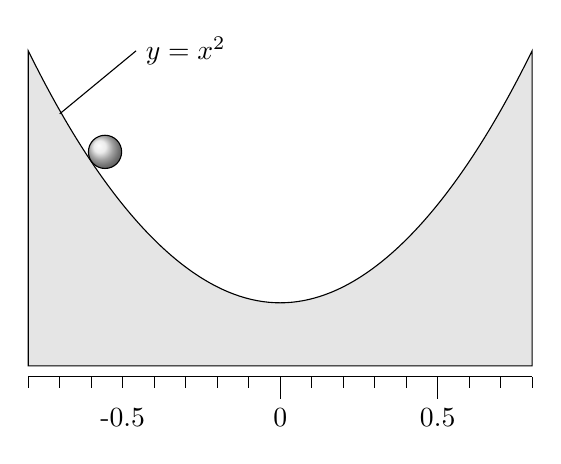
\begin{tikzpicture}[scale=0.4]
        %% accelerometer
        \draw[fill=white!90!black] (-8,0) -- (-8,10) parabola bend (0,2) (8,10) -- (8,0) -- cycle;
        %% label
        \node[anchor=center] (A) at (-3,10) {$y=x^2$};
        \draw (-7,8) -- (A.west);
        %% ball
        \draw[shading=ball,ball color=white!90!black] (-6,6.5) ++(33.69:1.5em) circle (1.5em);
        %% ruler
        \draw (-8,-1em) -- (8,-1em);
        \foreach \x in {-8,-7,...,8} {
            \draw (\x,-1em) -- (\x,-2em);
        }
        \foreach \x in {--5,0,5} {
            \draw (\x,-1em) -- (\x,-3em);
        }
        \node[anchor=north] at (-5,-3em) {\SI{-0.5}{\meter}};
        \node[anchor=north] at (0,-3em) {\SI{0}{\meter}};
        \node[anchor=north] at (+5,-3em) {\SI{0.5}{\meter}};
    \end{tikzpicture}
    \end{center}
    The device consists of a ball that is free to roll on a parabolic track.
    A scale along the bottom is used to measure the ball's horizontal position $x$.
    What is the acceleration of the car when the displacement of the ball in the accelerometer equals \SI{0.20}{\meter}?
    \begin{multicols}{2}
    \begin{choices}
      \correctchoice{\SI{3.9}{\meter\per\second\squared}}
        \wrongchoice{\SI{3.6}{\meter\per\second\squared}}
        \wrongchoice{\SI{26.5}{\meter\per\second\squared}}
        \wrongchoice{\SI{24.5}{\meter\per\second\squared}}
        \wrongchoice{\SI{9.1}{\meter\per\second\squared}}
    \end{choices}
    \end{multicols}
\end{question}
}



\endinput


